\documentclass{beamer}
\usepackage[english]{babel}

\usepackage[latin1]{inputenc}

\usepackage{graphicx}
% \usepackage{cmbright}
\usepackage{fancyvrb}
\usepackage{subfig}
\usepackage{caption}

\newsavebox{\mapss}
\newsavebox{\mapff}
\newsavebox{\mapnt}
\newsavebox{\maplocked}
\newsavebox{\mapstatic}

% Copyright 2004 by Till Tantau <tantau@users.sourceforge.net>.
%
% In principle, this file can be redistributed and/or modified under
% the terms of the GNU Public License, version 2.
%
% However, this file is supposed to be a template to be modified
% for your own needs. For this reason, if you use this file as a
% template and not specifically distribute it as part of a another
% package/program, I grant the extra permission to freely copy and
% modify this file as you see fit and even to delete this copyright
% notice. 
\mode<presentation>
{
  \usetheme{Amsterdam} % download from http://latex.simon04.net/beamerthemeAmsterdam.sty and put into the themes directory for beamer to use. You may need to run mktexlsr before you can compile it.
  %\usefonttheme{serif}
  % or ...

  \setbeamercovered{transparent}
  \beamertemplatenavigationsymbolsempty
  % or whatever (possibly just delete it)
}

\setbeamertemplate{footline}
{
  \leavevmode%
  \hbox{%
  \begin{beamercolorbox}[wd=.333333\paperwidth,ht=2.25ex,dp=1ex,center]{author in head/foot}%
    \usebeamerfont{author in head/foot}\insertshortauthor % Get rid of short institute next to name
  \end{beamercolorbox}%
  \begin{beamercolorbox}[wd=.333333\paperwidth,ht=2.25ex,dp=1ex,center]{title in head/foot}%
    \usebeamerfont{title in head/foot}\insertshorttitle
  \end{beamercolorbox}%
  \begin{beamercolorbox}[wd=.333333\paperwidth,ht=2.25ex,dp=1ex,right]{date in head/foot}%
    \usebeamerfont{date in head/foot}\insertshortdate{}\hspace*{2em}
    \insertframenumber{} / \inserttotalframenumber\hspace*{2ex} 
  \end{beamercolorbox}}%
  \vskip0pt%
}

% show sections at the start of each section
\AtBeginSection[]
{
  \begin{frame}
    \frametitle{Table of Contents}
    \tableofcontents[currentsection]
  \end{frame}
}

\makeatother
\setbeamercovered{dynamic}
\title[Sokoban] % (optional, use only with long paper titles)
{Sokoban: Search in a complex domain}

\author[Chazallon, Dossou-Gb{\'e}t{\'e}, Hong, Staniaszek]{Yann Chazallon,  Nicolas Dossou-Gb{\'e}t{\'e}, Tony Chan Ki Hong and Michal Staniaszek}

\setcounter{tocdepth}{1}

\date{\today}

% If you wish to uncover everything in a step-wise fashion, uncomment
% the following command: 

%\beamerdefaultoverlayspecification{<+->}

\begin{document}

\begin{frame}
  \titlepage
\end{frame}

\section{Introduction}

\begin{frame}{What is Sokoban?}
  Sokoban is a puzzle game first published in 1982
  \begin{itemize}
    \item The goal is to push boxes onto goal locations in a map
    \item Player can move up, down, left or right
    \item Boxes can only be pushed into empty spaces
    \item Can only move one box at a time
  \end{itemize}
\end{frame} 

\begin{frame}{Why is it interesting?}
  \begin{itemize}
  \item AI in games---investigate techniques in simple environments
  \item High branching factor comparable to chess, based on possible box moves
  \item Solution depth much deeper than any chess game
  \item Solutions can be arbitrarily long due to repeated motions
  \end{itemize}
\end{frame}

\section{Development Process}


\begin{lrbox}{\mapstatic}
  \begin{minipage}{.25\textwidth}
\centering
\begin{BVerbatim}
###XXXXX#######
#X#XXXXX#X210X#
#X#######6321X#
#Xcba98765432X#
#########XXXXX#
XXXXXXXX#######
\end{BVerbatim}
  \end{minipage}
\end{lrbox}%


\begin{frame}{Board Representation}
  \begin{columns}
    \begin{column}{.5\textwidth}
      \begin{itemize}
        \item Two layers
        \begin{itemize}
          \item Static (walls, goals): singleton
          \item Dynamic (player, boxes): search space
        \end{itemize}
        \item Static cost map calculated at launch
        \begin{itemize}
          \item Cost from each point to each goal
          \item Cost from each point to each initial box position
        \end{itemize}
      \end{itemize}
    \end{column}
    \begin{column}{.5\textwidth}
      \begin{block}{Static Lock and Cost Map}
        \centering
        \usebox{\mapstatic}
      \end{block}
    \end{column}
  \end{columns}
\end{frame}

\begin{frame}{Board hashing and equality}
  \begin{itemize}
    \item Hash: array of chars: \texttt{blank}, \texttt{\$} and \texttt{@}
    \item 2 versions: with and without player position
    \item Used for getHash(), getHashCode()
    \item 3 types of equality checks used:
    \begin{itemize}
      \item Without player position: check if state is goal
      \item With top leftmost player position: repeated state checks
      \item Exact player position: during the actual path reconstitution
    \end{itemize}
  \end{itemize}
\end{frame}

\begin{frame}{Heuristics}
  \begin{itemize}
    \item First heuristic: Manhattan distances
    \item Other unsuccessful attempts:
    \begin{itemize}
      \item Real cost
      \item Pseudo MinMatching
    \end{itemize}
  \end{itemize}
\end{frame}


\begin{frame}{Locked State Detection}
  \begin{columns}
    \begin{column}{.5\textwidth}
      \begin{itemize}
        \item Not using any pattern dictionary
        \item First implementation was building a graph of dependencies
        \item Then improved to explore implicit graph
        \item Should never return false positives
        \item Side-effect: able to detect corner locks (redundancy with static check)
      \end{itemize}
    \end{column}
    \begin{column}{.5\textwidth}
      \begin{block}{Dynamic Lock Test Map}
        \centering
        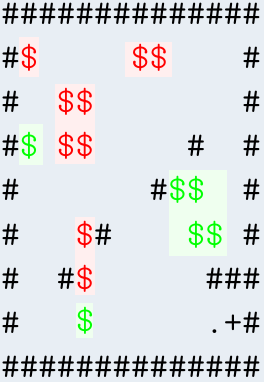
\includegraphics[width=0.6\textwidth]{dynamic.png}
      \end{block}
    \end{column}
  \end{columns}

\end{frame}

\begin{frame}{Player Space Search}
  Our first approach
  \begin{itemize}
  \item Successors of states based on the motions of the player
  \item Very slow---useless moves, even deeper solutions
  \item Applied A* search to find solutions
  \item Only trivial maps solved
  \end{itemize}
\end{frame}

\begin{frame}{Board Space Search}
  Improvement on the player space search
  \begin{itemize}
  \item Successors of states based on possible moves of accessible boxes
  \item Search changed to best-first search---don't need to find optimal solution
  \item BFS is complete, since we are using a closed list
  \item A* used to rebuild player path when a solution is found
  \item Managed to solve some nontrivial maps
  \end{itemize}
\end{frame}

\begin{frame}{Bi-directional Search}
  Our final version, improved search method rather than heuristics
  \begin{itemize}
  \item Previous attempts at improving heuristics failed
  \item Improving search seemed to be a better option
  \item Reduces the complexity from $\mathcal{O}(b^d)$ to $\mathcal{O}(b^{d/2})$
  \item Need to use multiple initial states for the reverse search
  \end{itemize}
\end{frame}

\begin{lrbox}{\mapff}
  \begin{minipage}{.25\textwidth}
\centering
\begin{BVerbatim}
###########
#  . . .  #
# . . . . #
####### x #
#    $ $  #
#       # #
###$####  #
#@ $   #$ #
### $  $  #
   ##     #
    #######  
\end{BVerbatim}
  \end{minipage}
\end{lrbox}%

\begin{lrbox}{\mapss}
  \begin{minipage}{.25\textwidth}
\centering
\small{
\begin{BVerbatim}
#########
##.$@ ###
###.# ###
###$#   #
#.$ #.# #
##.$ $# #
#.$ # # #
## #.$  #
#.$ #.###
##.$ $###
#.$ # ###
## $# ###
## .# ###
##    ###
#########
\end{BVerbatim}
}
  \end{minipage}
\end{lrbox}%

\begin{lrbox}{\mapnt}
  \begin{minipage}{.25\textwidth}
\centering
\small{
\begin{BVerbatim}
#################  
####    @##  #  #  
###   $ ##      #  
##   $ ##    ## ###
#   $ ##    ##  # #
#  $ ##    ##   $ #
# $ ##    ##  # # #
#  ##    ##  ## # #
#       ##  ### # #
####*  ##   ### # #
   #**##          #
   #######..*.#####
         ##...#    
          #####
\end{BVerbatim}
}
  \end{minipage}
\end{lrbox}%




\section{Evaluation}

\begin{frame}{Method Comparison}
  \begin{table}
    \centering
    \begin{tabular}{lccc}
      & \multicolumn{3}{c}{Time limit}\\
      \cline{2-4}
      Search Method              &  5 sec  &  11 sec  &  15 sec  \\
      \hline
      A*                         &     12  &      15  &      16  \\
      Best First                 &     56  &      60  &      64  \\
      Bi-directional Best First  &     76  &      81  &      82  \\
      Bi-directional A*          &     39  &      41  &      43  \\
    \end{tabular}
  \end{table}
  \begin{itemize}
  \item No significant difference in number of maps solved with different limits
  \item Is the search going in the right direction?
  \end{itemize}
\end{frame}

\begin{frame}{Map Performance}
  \begin{columns}
    \begin{column}{.5\textwidth}
       \begin{itemize}
       \item Can be solved within 15 sec, but not 11
       \item Requires a box to be positioned (at \texttt{x}) and not moved until the end.
       \item Problem is caused by heuristic preferring boxes on goals
       \end{itemize}
    \end{column}
    \begin{column}{.5\textwidth}
    \begin{block}{Map 54}
      \centering
      \usebox{\mapff}
    \end{block}
    \end{column}
  \end{columns}
\end{frame}

\begin{frame}{Map Performance}
  \begin{columns}
    \begin{column}{.5\textwidth}
      \begin{itemize}
      \item Solved very quickly
      \item All but one box require only a single move
      \item Heuristic gives accurate estimate to the goal
      \end{itemize}
    \end{column}
    \begin{column}{.5\textwidth}
      \begin{block}{Map 66}
        \centering
        \usebox{\mapss}
      \end{block}
    \end{column}
  \end{columns}
\end{frame}

\begin{frame}{Map Performance}
  \begin{columns}
    \begin{column}{.5\textwidth}
      \begin{itemize}
      \item Unsolved within 15 sec
      \item Intermediate goal area causes issues with heuristic
      \item Requires making specific move sequences to get boxes on goals
      \end{itemize}
    \end{column}
    \begin{column}{.5\textwidth}
      \begin{block}{Map 93}
        \centering
        \usebox{\mapnt}
      \end{block}
    \end{column}
  \end{columns}
\end{frame}

\section{Conclusions}
\begin{frame}{Reflection and Conclusions}
  \begin{itemize}
  \item Focussed more on search than heuristic
  \item Did not consider memory requirements---could improve map representation
  \item Took a long time to get a simple solver
  \item A* is good, but application dependent
  \end{itemize}
\end{frame}

\begin{frame}{Questions}
  \begin{center}
    \Huge{?}
  \end{center}

\end{frame}

\end{document}
